Over the course of this review it has become obvious that more and earlier data would provide the next steps for both progenitor channel and correlation constraining of SNe Ia with host properties. If more SNe Ia in hosts can be collected and much earlier before peak flux, then the correlations with host galaxy properties can be more easily studied which enables improvements for standardisation methods. 

The EEx SNe Ia are difficult to find, with most studies not being population studies but rather case studies, and the few population studies result in a sample size of 6 and 3 \parencite{deckers_constraining_2022, burke_early_2022, wu_wfst_2026}. The Vera C. Rubin Observatory which will be referred to as Rubin from here on out, is located in El Peñón peak of Cerro Pachón in Chile \parencite{bianco_optimization_2022}. The observatory hosts a 8.36 metre aperture and will have filters across a wavelength range of 320.5 nanometres to 1084.5 nanometres \parencite{bianco_optimization_2022}. The viewing cadence of LSST has an average revisit time of 3 days across the whole southern sky which, covers an area of 18000 $deg^2$ which gives the median number of revisits at 825 per site \parencite{bianco_optimization_2022, ivezic_lsst_2019}. As can be seen in Figure \ref{fig: Map of the fields that Rubin will visit with the median number of revists across different portions of the Southern Sky.} Some portions of the Southern Sky will be visited more than others but the main Wide-Fast-Deep (WFD) survey will have an average of 900 revisits across the 10 years that LSST will operate over.   

\begin{figure}[htbp]
    \centering
    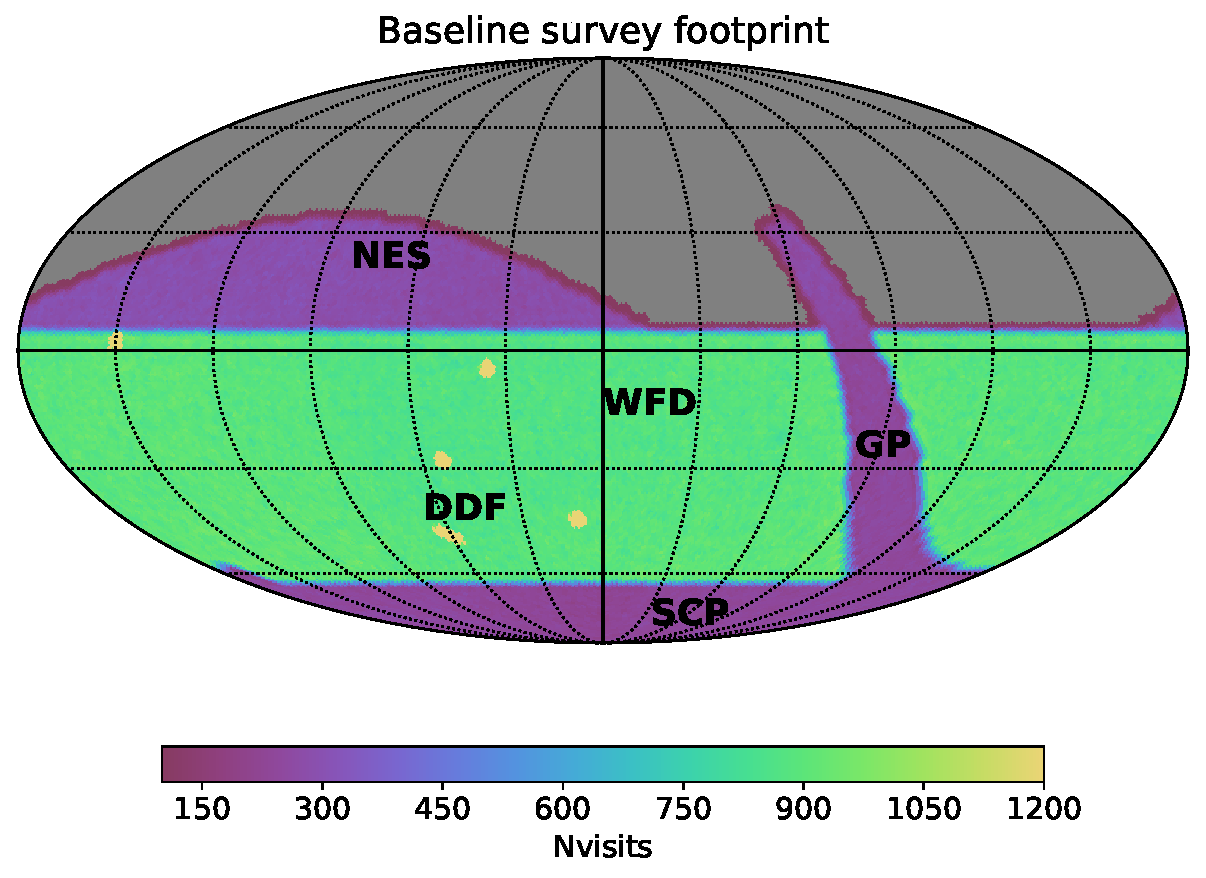
\includegraphics[width=0.65\linewidth]{graphics/Fink_Rubin_LSST/baseline_nexp2_v171_10yrs_nvisits.pdf}
    \caption{The baseline number of visits that Rubin will make across the Southern Sky. Taken from \textcite{bianco_optimization_2022}, the different areas on the map show the main survey, WFD, and additional mini surveys. With NES being the North Ecliptic Spur, DDF represents the Deep Drilling Fields, GP is the Galactic Plane and SCP is the South Celestial Pole. It is easy to see that different surveys using the Rubin Observatory require different viewing cadences to enable the collection of data that is desired.}
    \label{fig: Map of the fields that Rubin will visit with the median number of revists across different portions of the Southern Sky.}
\end{figure}

Over the course of the survey the expected number of alerts generated each night will be 10 million per night and within 60 seconds, transients will be reported \parencite{moller_fink_2021}. Of these alerts it is expected that there will be $\approx 1100$ SNe per night. This should enable the opportunity to discover more SNe Ia which will increase the odds of finding the EEx SNe Ia and could enable the beginnings of a population study with respect to their host galaxy properties. 

To handle this number of alerts, we employ the use of the Fink broker which allows for the processing of the large number of alerts from the alert stream of Rubin. Fink does the ingestion of the data of the LSST alert stream, annotation of the alerts such as early light curve classification and is capable of customisable filtering of the alerts \parencite{moller_fink_2021}. 

Fink employs machine learning methods of classification to disentangle the types of SNe that will be discovered by Rubin. These machine learning classifiers use an active learning approach that can take a smaller sample of training data and continually retrain the classification models to improve the models as the survey progresses in time\parencite{leoni_fink_2022}. This means that SNe Ia will be readily classified from the LSST alert stream producing science-ready images in mere minutes. 